\section{Propuesta de arquitectura de datos}

La arquitectura usa una única instancia de PostgreSQL para los datos
operativos, los metadatos documentales, los embeddings, los permisos, las
consultas, las respuestas y la auditoría. Las extensiones \texttt{pgvector} y
\texttt{btree\_gist} incorporan búsqueda vectorial y restricciones temporales
sin agregar otro motor.

El motor único permite combinar relaciones estructuradas, vigencia,
autorización y similitud en una misma consulta. Separar la base relacional de
la vectorial exigiría duplicar metadatos y sincronizarlos, sin aportar una
ventaja comprobable para el volumen de esta prueba.

La Figura~\ref{fig:arquitectura} resume el recorrido. El generador produce el
SQL de datos, los documentos Markdown y un manifiesto con conteos, checksums y
oráculos. El cargador ejecuta el esquema, los datos, los índices, las vistas y
la seguridad. Una aplicación futura podrá consultar la base mediante el rol de
ejecución; el frontend, la API y la integración con un LLM quedan fuera de la
implementación mínima.

\begin{figure}[htbp]
\centering
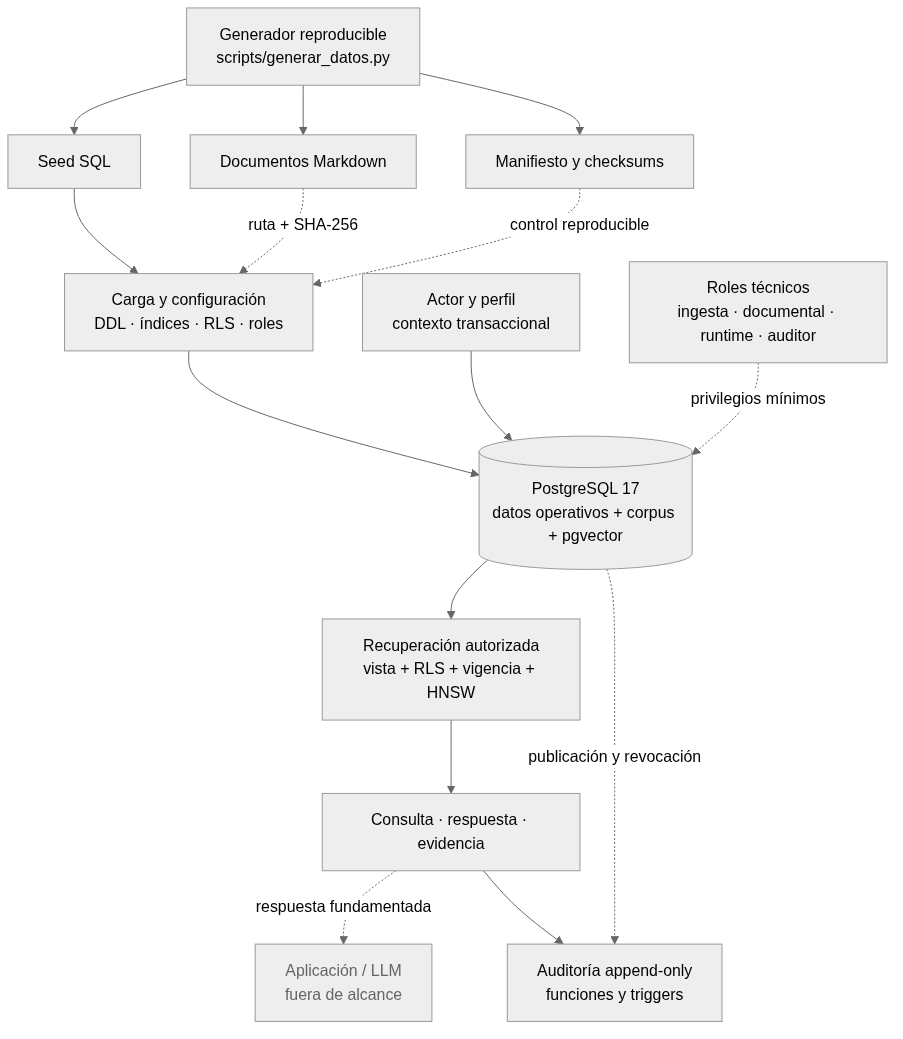
\includegraphics[width=\textwidth,height=0.78\textheight,keepaspectratio]{arquitectura.png}
\caption{Arquitectura general y recorrido de los datos.}
\label{fig:arquitectura}
\end{figure}
\FloatBarrier

Los documentos permanecen fuera de PostgreSQL. La base conserva su ruta
relativa, procedencia, tamaño, tipo MIME y checksum. Esta separación evita
guardar archivos en tablas y permite trasladarlos en el futuro a almacenamiento
de objetos sin cambiar el contrato de integridad.

No se incorpora un Data Warehouse, Data Lake o Lakehouse porque las consultas
son operativas y el conjunto de datos es pequeño. Si el sistema necesitara
análisis históricos o reportes a otra escala, los hechos y eventos podrían
extraerse hacia una capa analítica separada.
